\documentclass{beamer}
\usetheme{Boadilla}
\usecolortheme{beaver}

\usepackage[german]{babel}
\usepackage[utf8x]{inputenc}
\usepackage{tabularx}
\usepackage{slashbox}
\usepackage{tikz}
\usetikzlibrary{mindmap,trees}

\title[Collaborative \& transparent FS development]{Collaborative and transparent Free Software development} 
\author{Lydia Pintscher} 
\institute[KIT]{Institute of Applied Informatics and Formal Description Methods\\
Karlsruhe Institute of Technology
}
\date{30. Juni 2011}

\begin{document}
\begin{frame}
\titlepage
\end{frame}

%\section{Einleitung}

\begin{frame}
%\frametitle{Einleitung}
\begin{itemize}
 \item Freie Software = integraler Bestandteil der Technologiewelt
 \item sehr unterschiedliche Projekte mit \"ahnlichen Problemen: Amarok und Halo
 \item mehr Transparenz und Kollaboration
 \item Analyse und Verbesserung des Entwicklungsprozesses mit vertrauten Tools
\end{itemize}
\end{frame}

\section*{\"Ubersicht}

\begin{frame}
\frametitle{\"Ubersicht}
\tableofcontents
\end{frame}

\AtBeginSection[]
{
\begin{frame}
\frametitle{\"Ubersicht}
\tableofcontents[currentsection]
\end{frame}
}

\section{Grundlagen}

\begin{frame}
\frametitle{Kollaboration und Transparenz}
\begin{itemize}
 \item Kollaboration: ``working jointly with others or together especially in an intellectual endeavour'' (Merriam-Webster)
 \item Transparenz (hier): einfacher Zugang zu und Sichtbarkeit von Informationen 
\end{itemize}
\end{frame}

\begin{frame}
\frametitle{Freie Software (1)}
\begin{itemize}
 \item beschreibt eine Philosophie zum Entwickeln und Verbreiten von Software
 \item bekannnte Beispiele: Apache http Server, Firefox, MediaWiki
\end{itemize}
\end{frame}

\begin{frame}
\frametitle{Freie Software (2)}
\begin{itemize}
 \item verschiedene Projektformen (volunteer $\leftrightarrow$ company)
 \item verschiedene Gr\"unde teilzuhaben (extrinsisch $\leftrightarrow$ intrinsisch)
 \item unterschiedlich gro\ss e gef\"uhlte Distanz zwischen Mitgliedern
 \item unterschiedliche Arbeits- und Kommunikationsstile
\end{itemize}

\begin{block}{Spektrum der bestimmenden Kr\"afte in einem Freien Software Projekt}
\begin{figure}[h]
	\centering
	\begin{tikzpicture}
		\draw (0cm, 0cm) -- (10cm, 0cm);
		\foreach \x in {0, 1, 2, 3, 4, 5, 6, 7, 8, 9, 10} \draw (\x cm, 3pt) -- (\x cm, - 3pt);
		\draw (0cm, 0cm) node[below=5pt] {ehrenamtlich};
		\fill (0.625cm, 0cm) circle (2pt);\draw (0.625cm, 0cm) node[above=5pt] {Amarok};
		\draw (5cm, 0cm) node[below=5pt] {gemischt};
		\fill (8.75cm, 0cm) circle (2pt);\draw (8.75cm, 0cm) node[above=5pt] {Halo};
		\draw (10cm, 0cm) node[below=5pt] {bezahlt};
	\end{tikzpicture}
\end{figure}
\end{block}
\end{frame}

\begin{frame}
\frametitle{Halo}
\begin{itemize}
 \item Erweiterungen f\"ur Semantic MediaWiki
 \item Vereinfachung und Erweiterung der Nutzung semantischer Daten in einem Wiki
 \item Hauptaugenmerk auf Nutzung im Gesch\"aftsumfeld
 \item sehr starker Einfluss von Hauptsponsor Vulcan Inc.
 \item Atmosph\"are in der Community stark gekennzeichnet von kommerziellem Einfluss
\end{itemize}
\end{frame}

\begin{frame}
\frametitle{Amarok}
\begin{itemize}
 \item Musikabspielprogramm aus der KDE Community
 \item fast ausschlie\ss lich ehrenamtlich entwickelt
 \item Motto: rediscover your music
 \item verteiltes Team - Kommunikation \"uber IRC und Mailinglisten
 \item sehr flache Teamstruktur
\end{itemize}
\end{frame}

\section{Analyse}

\begin{frame}
\frametitle{Vorgehensweise}
\begin{itemize}
 \item strukturierte, vertrauliche Interviews
     \begin{itemize}
        \item Wer sind die Beteiligten?
        \item Welche Tools werden benutzt?
        \item Welche Probleme m\"ussen bew\"altigt werden?
     \end{itemize}
 \item Auswahl der Teilnehmer basierend auf ihrer Zeit im Projekt und ihrem T\"atigkeitsbereich
\end{itemize}
\begin{figure}[h!]
 \centering
 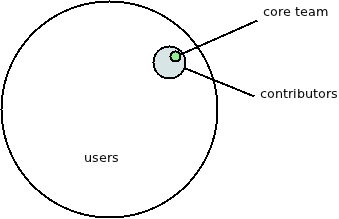
\includegraphics[scale=0.35,keepaspectratio=true]{./communitymodel.png}
\end{figure}
\end{frame}

\begin{frame}
\frametitle{Communitymodell}
\begin{figure}[h!]
 \centering
 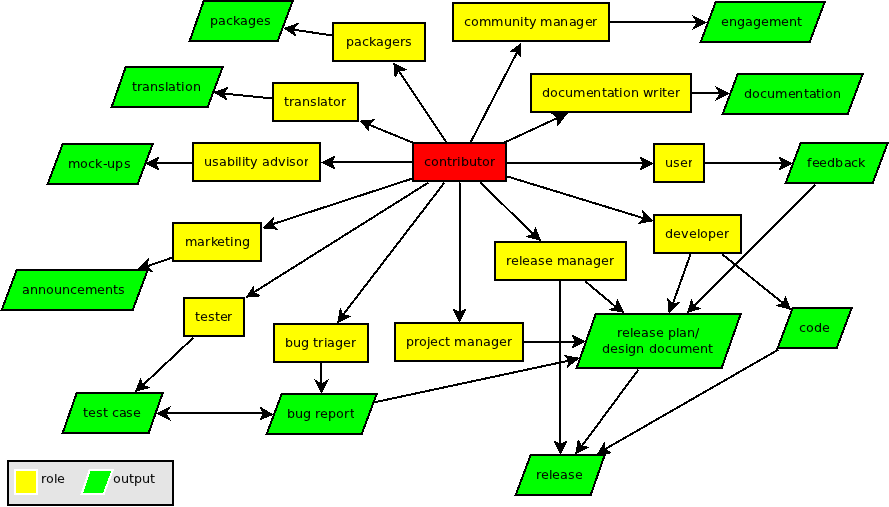
\includegraphics[scale=0.35,keepaspectratio=true]{./ontology.png}
\end{figure}
\end{frame}

\begin{frame}
\frametitle{Halo - Releaseprozess}
\begin{figure}[h!]
 \centering
 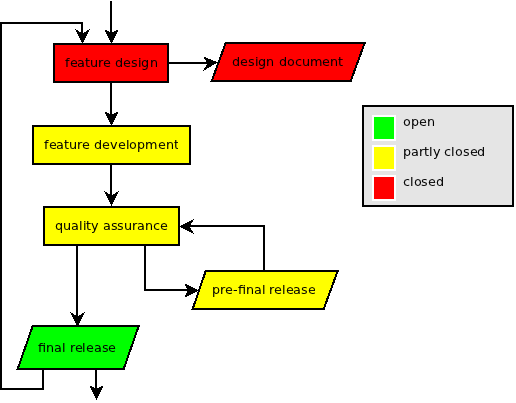
\includegraphics[scale=0.5,keepaspectratio=true]{./ReleaseProcessHalo.png}
\end{figure}
\end{frame}

\begin{frame}
\frametitle{Halo - Aktivit\"aten}
\begin{center}
\begin{tikzpicture}
  \path[small mindmap, concept color=green, text=black]
    node[concept] {Aktivit\"aten Halo}
    [clockwise from=0]
    child[concept color=green!80, grow=0] {
      node[concept] {Feature Design}
    }  
    child[concept color=green!80, grow=60] {
      node[concept] {Code schreiben}
    }
    child[concept color=green!80, grow=120] {
      node[concept] {Qua\-li\-t\"ats\-sich\-er\-ung}
    }  
    child[concept color=green!80, grow=180] {
      node[concept] {Nutz\-er\-ein\-be\-zieh\-ung und Support}
    }
    child[concept color=green!80, grow=240] {
      node[concept] {Ein\-be\-zieh\-ung der Con\-tri\-bu\-tor}
    }  
    child[concept color=green!80, grow=300] {
      node[concept] {Promotion}
    };
\end{tikzpicture}
\end{center}
\end{frame}

\begin{frame}
\frametitle{Halo - Probleme}
\begin{center}
\begin{tikzpicture}
  \path[small mindmap, concept color=green, text=black]
    node[concept] {Probleme Halo}
    [clockwise from=0]
    child[concept color=green!80, grow=0] {
      node[concept] {Kom\-mu\-ni\-ka\-tion von Vision/Ziel}
    }  
    child[concept color=green!80, grow=90] {
      node[concept] {Ko\-or\-di\-na\-tion der QA}
    }
    child[concept color=green!80, grow=180] {
      node[concept] {Trans\-pa\-renz und Ko\-or\-di\-na\-tion}
    }  
    child[concept color=green!80, grow=270] {
      node[concept] {Nutzer\-input}
    };
\end{tikzpicture}
\end{center}
\end{frame}

\begin{frame}
\frametitle{Amarok - Releaseprozess}
\begin{figure}[h!]
 \centering
 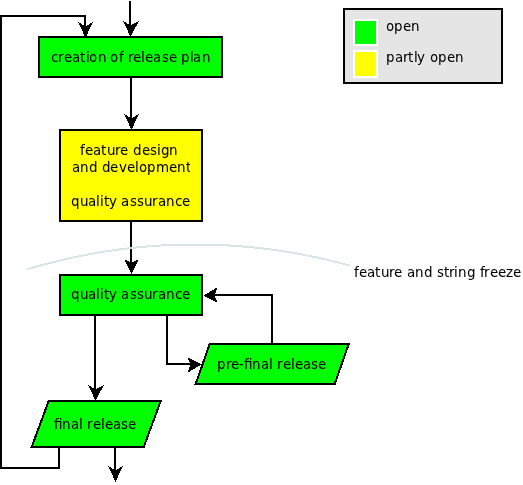
\includegraphics[scale=0.43,keepaspectratio=true]{./ReleaseProcessAmarok.png}
\end{figure}
\end{frame}

\begin{frame}
\frametitle{Amarok - Aktivit\"aten}
\begin{center}
\begin{tikzpicture}
  \path[small mindmap, concept color=blue, text=white]
    node[concept] {Aktivit\"aten Amarok}
    [clockwise from=0]
    child[concept color=blue!80, grow=0] {
      node[concept] {Release Management}
    }  
    child[concept color=blue!80, grow=60] {
      node[concept] {Code schreiben}
    }
    child[concept color=blue!80, grow=120] {
      node[concept] {Qua\-li\-t\"ats\-sich\-er\-ung}
    }  
    child[concept color=blue!80, grow=180] {
      node[concept] {Nutz\-er\-ein\-be\-zieh\-ung und Support}
    }
    child[concept color=blue!80, grow=240] {
      node[concept] {Team\-ein\-be\-zieh\-ung und Management}
    }  
    child[concept color=blue!80, grow=300] {
      node[concept] {Promotion}
    };
\end{tikzpicture}
\end{center}
\end{frame}

\begin{frame}
\frametitle{Amarok - Probleme}
\begin{center}
\begin{tikzpicture}
  \path[small mindmap, concept color=blue, text=white]
    node[concept] {Probleme Amarok}
    [clockwise from=0]
    child[concept color=blue!80, grow=0] {
      node[concept] {klare Vision/Ziel}
    }  
    child[concept color=blue!80, grow=90] {
      node[concept] {Roadmap}
    }
    child[concept color=blue!80, grow=180] {
      node[concept] {Trans\-pa\-renz und Ko\-or\-di\-na\-tion}
    }  
    child[concept color=blue!80, grow=270] {
      node[concept] {Ko\-or\-di\-na\-tion der QA}
    };
\end{tikzpicture}
\end{center}
\end{frame}

\section{Design}

\begin{frame}
\frametitle{Anforderungen, Erwartungen und Rahmenbedingungen}
\begin{itemize}
 \item Vertrauen aufbauen durch Transparenz
 \item schnellen \"Uberblick und Beitr\"age gew\"ahren
 \item ``cookie licking'' vermeiden
 \item keine Zeit verschwenden
 \item Freie Software nutzen
 \item Erwartungen richtig setzen
 \item Einstellungen \"andern
\end{itemize}
\end{frame}

\begin{frame}
\frametitle{Kollaborativ in einem Team arbeiten}
\begin{itemize}
 \item Team- und Aufgabenbewusstsein
 \item Zeitplan f\"ur Releases
 \item Code ownership
 \item Checklisten
 \item Vertrauen aufbauen durch Einbeziehen
 \item Commits verkn\"upfen
\end{itemize}
\end{frame}

\begin{frame}
\frametitle{Kollaborativ an einer Vision arbeiten}
\begin{itemize}
 \item Erstellen und Kommunizieren einer Vision
 \item Kollaborativ eine Vision aktualisieren
\end{itemize}
\end{frame}

\begin{frame}
\frametitle{Kollaborativ eine Roadmap erstellen (1)}
\begin{columns}
 \column{.4\textwidth}
  \begin{itemize}
   \item Lebenszyklus eines feature requests
   \item Umfang und Schwierigkeit von feature requests
   \item Erwartungen um einen feature request kommunizieren
   \item Annehmen und Zuweisen von feature requests
   \item Seite f\"ur feature request und \"Ubersicht
  \end{itemize}
 \column{.6\textwidth}
  \begin{figure}[h!]
   \centering
   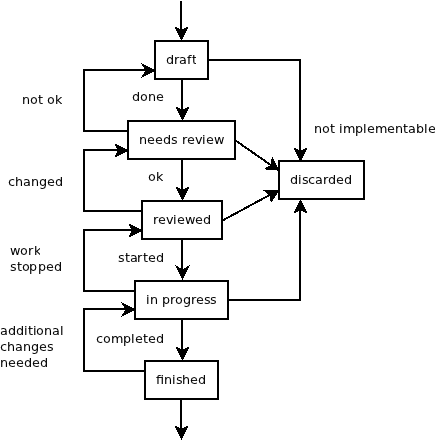
\includegraphics[scale=0.4,keepaspectratio=true]{./featurerequeststates.png}
  \end{figure}
\end{columns}
\end{frame}

\begin{frame}
\frametitle{Kollaborativ eine Roadmap erstellen (2)}
\begin{table}[h]
\begin{tabular}{|p{0.1\textwidth}|p{0.8\textwidth}|}
\hline
Priorit\"at & Bedeutung\\
\hline \hline
P1 & wird vom core team implementiert werden\\
\hline
P2 & wird vielleicht vom core team implementiert werden\\
\hline
P3 & wird nicht vom core team implementiert werden aber patches sind gern gesehen\\
\hline
P4 & unentschieden oder kontrovers\\
\hline
P5 & wird nicht implementiert werden und patches werden wahrscheinlich nicht akzeptiert werden\\
\hline
\end{tabular}
\centering
\end{table}
\end{frame}

\begin{frame}
\frametitle{Kollaborativ eine Roadmap erstellen (3)}
\begin{table}[h]
\begin{tabular}{|l||*{4}{c|}}
\hline
\backslashbox{Umfang}{Schwierigkeit}&\makebox[3em]{leicht}&\makebox[3em]{mittel}&\makebox[3em]{schwer}\\
\hline \hline
klein & 1 & 3 & 6\\
\hline
mittel & 2 & 5 & 8\\
\hline
gro\ss & 4 & 7 & 9\\
\hline
\end{tabular}
\centering
\end{table}
\end{frame}

\begin{frame}
\frametitle{Qualit\"atssicherung}
\begin{itemize}
 \item Testen durch eine gr\"o\ss ere Gruppe f\"ordern
 \item Problembereiche sichtbarer machen
\end{itemize}

\begin{figure}[h]
 \centering
 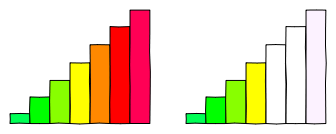
\includegraphics[scale=0.6,keepaspectratio=true]{./activityindicator.png}
\end{figure}
\end{frame}

\begin{frame}
\frametitle{Bausteine}
\begin{figure}[h]
 \centering
 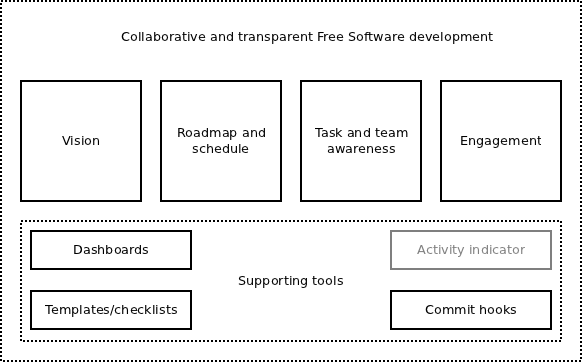
\includegraphics[scale=0.5,keepaspectratio=true]{./buildingblocks.png}
\end{figure}
\end{frame}

\section{Implementierung}

\begin{frame}
\frametitle{Einf\"uhrungsszenario}
\begin{itemize}
 \item nacheinander, unabh\"angig voneinander um zu sehen, wie es angenommen wird
 \item meist erst f\"ur Amarok und dann Halo
\end{itemize}
\end{frame}

\begin{frame}
\frametitle{Kommunikation und Kollaboration in einem verteilten Team}
\begin{columns}
 \column{.5\textwidth}
   \begin{itemize}
     \item team dashboard
     \item release dashboard
     \item code ownership
     \item checklists
   \end{itemize}
 \column{.5\textwidth}
   \begin{figure}
     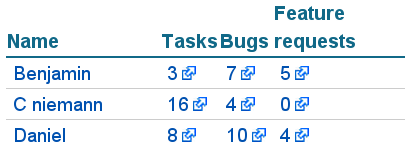
\includegraphics[scale=0.4,keepaspectratio=true]{./TeamDashboardTable.png}
   \end{figure}
\end{columns}
   \begin{figure}
     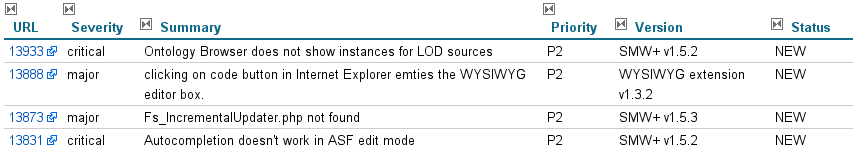
\includegraphics[scale=0.45,keepaspectratio=true]{./bugListHalo.png}
   \end{figure}
\end{frame}

\begin{frame}
\frametitle{Kollaborativ an einer Vision arbeiten}
\begin{block}{Amaroks neue Vision}
\begin{quotation}``The Amarok team strives to develop a free and open music player that is innovative and powerful, yet easy to use. Amarok helps rediscover music by giving access to a vast amount of different music sources and related information. In a world where music and computing are everywhere, Amarok aims to provide the best music listening experience anywhere, anytime. The Amarok team promotes free culture. Amarok makes people happy.''\end{quotation}
\end{block}
\end{frame}

\begin{frame}
\frametitle{Kollaborativ eine Roadmap erstellen (1)}
\begin{itemize}
 \item 2 Feature Tracking Systeme
 \begin{itemize}
   \item einfaches MediaWiki template f\"ur Amarok
   \item Semantic Form f\"ur Halo
 \end{itemize}
\end{itemize}
\begin{figure}
 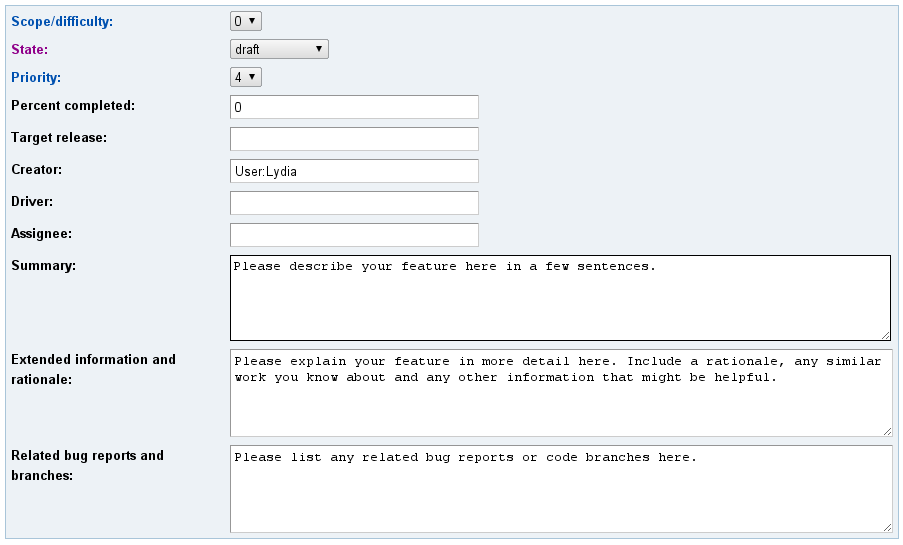
\includegraphics[scale=0.25,keepaspectratio=true]{./featuretrackingform.png}
\end{figure}
\end{frame}

\begin{frame}
\frametitle{Kollaborativ eine Roadmap erstellen (2)}
\begin{figure}
 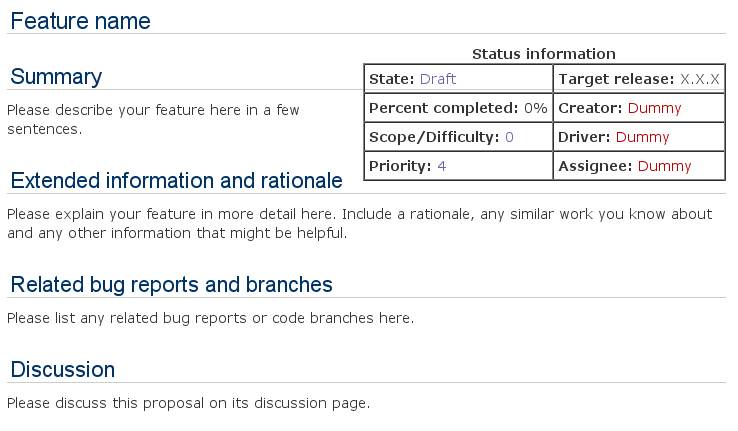
\includegraphics[scale=0.45,keepaspectratio=true]{./FeatureProposalTemplateAmarok.png}
\end{figure}
\end{frame}

\begin{frame}
\frametitle{Qualit\"atssicherung}
\begin{itemize}
 \item Testcheckliste
 \item Public Testing Contest
 \item Emails von Bugzilla
\end{itemize}
\end{frame}

\section{Evaluation}

\begin{frame}
\frametitle{Umfrage (1)}
\begin{columns}
 \column{.5\textwidth}
   ``Wird das team dashboard die Transparenz erh\"ohen?''
   \begin{figure}[h!]
    \centering
    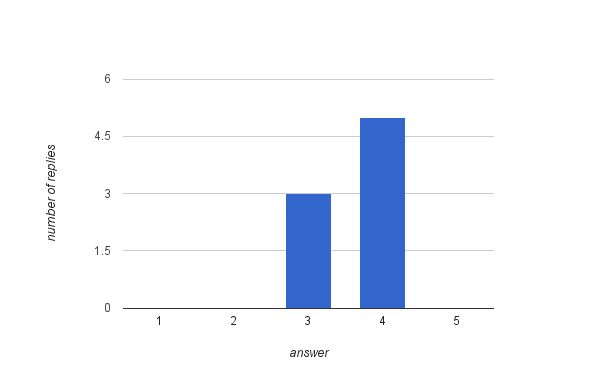
\includegraphics[scale=0.3,keepaspectratio=true]{./halo2a.png}
   \end{figure}
 \column{.5\textwidth}
   ``Wird das release dashboard die Transparenz erh\"ohen?''
   \begin{figure}[h!]
    \centering
    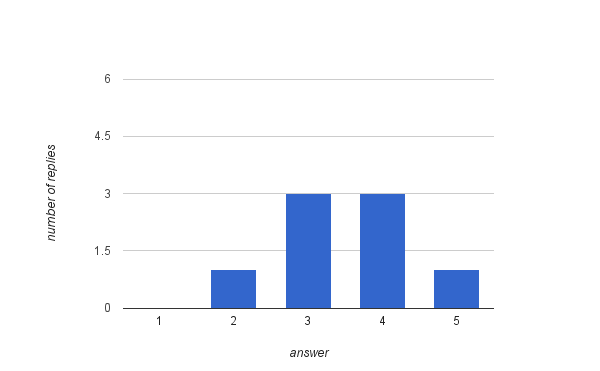
\includegraphics[scale=0.3,keepaspectratio=true]{./halo2d.png}
   \end{figure}
\end{columns}
\end{frame}

\begin{frame}
\frametitle{Umfrage (2)}
\begin{columns}
 \column{.5\textwidth}
   ``Glaubst du, dass der Prozess zur Entwicklung der neuen Vision transparent/kollaborativ war?''\newline
   \begin{figure}[h!]
    \centering
    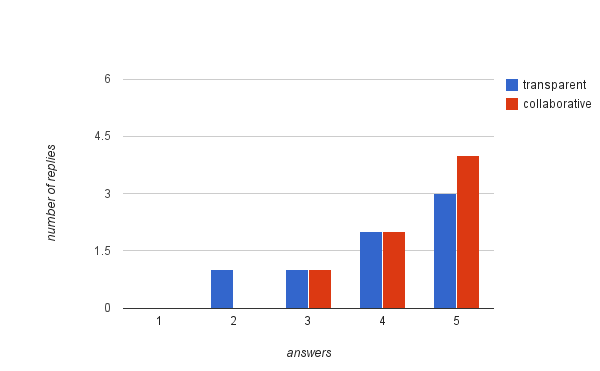
\includegraphics[scale=0.25,keepaspectratio=true]{./amarok1ef.png}
   \end{figure}
 \column{.5\textwidth}
   ``Glaubst du, dass der Prozess zur Entwicklung der neuen Vision auch von anderen Freien Software Projekten genutzt werden kann?''
   \begin{figure}[h!]
    \centering
    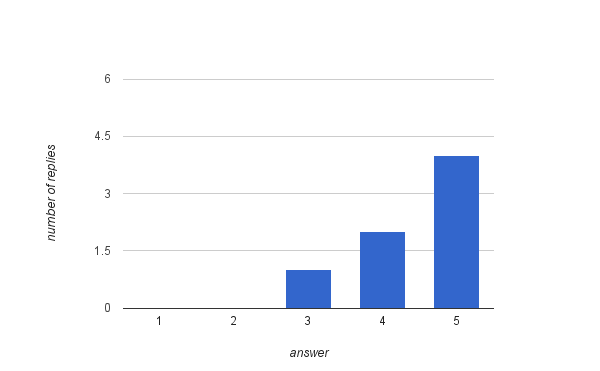
\includegraphics[scale=0.25,keepaspectratio=true]{./amarok1d.png}
   \end{figure}
\end{columns}
\end{frame}

\begin{frame}
\frametitle{Umfrage (3)}
\begin{columns}
 \column{.5\textwidth}
  ``Wird das neue feature tracking form/template die Kollaboration zwischen Contributorn/Contributorn und Nutzern verbessern?''
   \begin{figure}[h!]
    \centering
    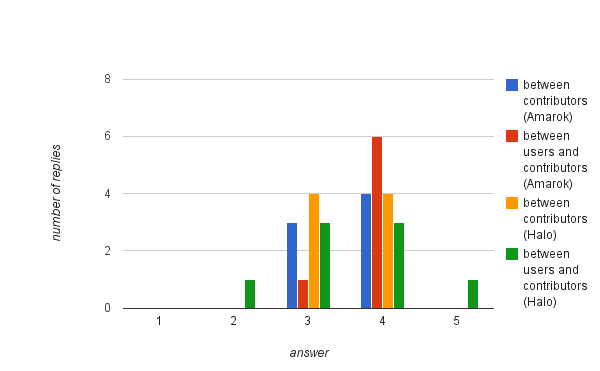
\includegraphics[scale=0.25,keepaspectratio=true]{./amarok3bchalo3bc.png}
   \end{figure}
 \column{.5\textwidth}
 ``Wird das neue feature tracking form/template und die roadmap die Transparenz erh\"ohen?''\newline
   \begin{figure}[h!]
    \centering
    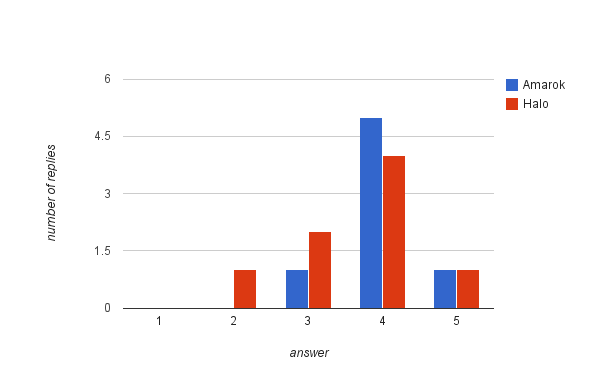
\includegraphics[scale=0.25,keepaspectratio=true]{./amarok3dhalo3d.png}
   \end{figure}
\end{columns}
\end{frame}

\begin{frame}
\frametitle{Ver\"anderung in der Offenheit des Entwicklungsprozesses}
\begin{columns}[t]
 \column{.5\textwidth}
   \begin{center}Halo\end{center}
   \begin{figure}[h!]
    \centering
    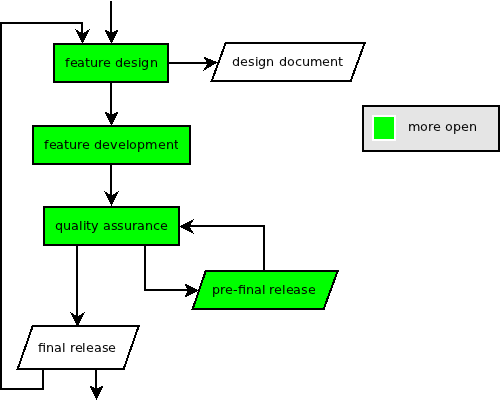
\includegraphics[scale=0.3,keepaspectratio=true]{./ReleaseProcessHaloNew.png}
   \end{figure}
 \column{.5\textwidth}
   \begin{center}Amarok\end{center}
   \begin{figure}[h!]
    \centering
    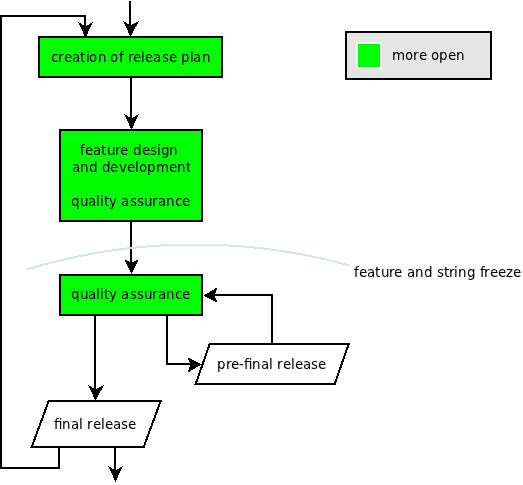
\includegraphics[scale=0.3,keepaspectratio=true]{./ReleaseProcessAmarokNew.png}
   \end{figure}
\end{columns}
\end{frame}

\section{Zusammenfassung und Ausblick}

\begin{frame}
\frametitle{Zusammenfassung und Ausblick}
\begin{itemize}
 \item 2 Projekten geholfen ihren Entwicklungsprozess offener und kollaborativer zu gestalten
 \item wichtige Fragen f\"ur die Zukunft der Projekte gestellt auch wenn diese nicht immer angenehm waren
 \item Werkzeuge und Prozesse entwickelt die auch von anderen Freien Software Projekten genutzt werden k\"onnen weil sie im Einklang sind mit der Arbeitsweise eines Freien Software Projektes
 \item in Zukunft sollten Tests mit anderen Projekten durchgeführt werden und der Activity Indicator implementiert werden
\end{itemize}
\end{frame}

\begin{frame}
\begin{center}
 Vielen Dank f\"ur ihre Aufmerksamkeit.
\end{center}

\begin{columns}
 \column{.5\textwidth}
   \begin{figure}[h!]
    \centering
    
\includegraphics[scale=0.5,keepaspectratio=true]{./smwpluslogo.png}
   \end{figure}
 \column{.5\textwidth}
   \begin{figure}[h!]
    \centering
    
\includegraphics[scale=0.3,keepaspectratio=true]{./amaroklogo.png}
   \end{figure}
\end{columns}
\end{frame}

\begin{frame}
\frametitle{Die 4 Freiheiten}
\begin{block}{4 Freiheiten Freier Software (Free Software Foundation)}
    Die Freiheit, \dots
    \begin{enumerate}
      \item das Programm für jeden Zweck zu benutzen.
      \item zu verstehen, wie das Programm funktioniert und wie man es für seine Ansprüche anpassen kann.
      \item Kopien weiterzuverbreiten, so dass man seinem Nächsten weiterhelfen kann.
      \item das Programm zu verbessern und die Verbesserungen der Öffentlichkeit zur Verfügung zu stellen, damit die ganze Gemeinschaft davon profitieren kann.
    \end{enumerate}
\end{block}
\end{frame}

\begin{frame}
\frametitle{Vergleich und Schlussfolgerung (1)}
\begin{tabularx}{\textwidth}{|X|X|X|}
\hline
 & Halo & Amarok \\
\hline \hline
Alter & 2 Jahre & 7 Jahre \\
\hline
Programmiersprache & PHP & C++ \\
\hline
Motivation & vorw. extrinsisch & vorw. intrinsisch \\
\hline
Teamgrenzen & klar & unklar\\
\hline
haupts\"achlich genutzte Medien & pers\"onlich, Mailinglisten, Bugreports & IRC, Mailinglisten \\
\hline
Community au\ss erhalb des Kernteams & klein & gro\ss \\
\hline
Offenheit & rel. geschlossen & rel. offen \\
\hline
``release early release often'' & nein & ja \\
\hline
Planung & viel & sehr wenig \\
\hline
Richtungsvorgabe & Management/Team & individuelle Entwickler \\
\hline
Standort Kernteam & Deutschland & weltweit \\
\hline
\end{tabularx}
\end{frame}

\begin{frame}
\frametitle{Vergleich und Schlussfolgerung (2)}
\begin{tabularx}{\textwidth}{|X|X|X|}
\hline
 & Halo & Amarok\\
\hline \hline
Versionskontrollsystem & SVN & git\\
\hline
wiki & MediaWiki, SMW und Halo & MediaWiki\\
\hline
bug tracker & Bugzilla & Bugzilla\\
\hline
build server & Hudson & Hudson\\
\hline
test case management & TestLink & Seite im wiki\\
\hline
\end{tabularx}
\end{frame}

\end{document}
